\chapter{Evaluation of Estimation Methods}

When estimating Respiratory Rate from ECG signal, the common approach is to isolate RR peaks, and then work with the 
waveform associated with amplitude and time of the RR peaks \cite{MIRMOHAMADSADEGHI201466}. There are two common methods; the first focuses on locating 
the dominate frequency in the time between RR peaks, this corresponds to the biological phenomenon of 
Respiratory Sinus Arrhythmia (RSA), which states that heart rate speeds up when you breath in and slows down when you breath out
\cite{clevelandclinic_sinus_arrhythmia}, \cite{MIRMOHAMADSADEGHI201466}. The data we are working with here is 2D, with each pair corresponding 
to the length of time between RR peaks and the midpoint of that time interval. The other method is based on the amplitude differences of the RR peaks (RPA),
which is associated to impacts breathing in and out has on the electrical output of the heart \cite{MIRMOHAMADSADEGHI201466}. The 
data we are working with here is similarily 2D with each pair corresponding to the amplitude of Peak and the time at which it occured.
The idea behind both methods is to then isolate the frequency with the strongest associated amplitude, where 
the assumption is that this frequency corresponds to the  Respiratory Rate whilst the less dominate frequencies correspond to noise 
and other biological processes and artifacts. The normal Respirate Rate range is 12 - 20 BPM \cite{chourpiliadis2022respiratory}, which corresponds to a range of  0.2- 0.33Hz , for a candidate
Respiratory Rate. Note that we can't ignore frequencies outside of the range especially as we know we are dealing with data where Apnea and possible
other Respiratory events are occuring that cause Respiratory Rate to land outside of the normal range - hence we a predominantly looking for a consistent
dominate frequency  within a range of 0.05 - 0.50 Hz (to avoid noise). In all of the work below, the RR peaks are identified 
using the Jump Detection Algorithm described above.  

\section{Spectrum Analysis Methods}
Implementing either of these methods requires spectrum analysis, however as we are dealing with non-uniform time data we can't blindly
apply the Fast Fourier Transform (FFT). There are two ways of dealing with non-uniform time series data which we explore in 
this project. The first is to use an interpolation method between the RR peaks and then sample a uniform time 
from this and apply FFT to this waveform, the other is to use the Lomb-Scargle Method defined for non-uniform time 
series data. We give a brief explanation of each method, and compare the output spectrum of those in this section, then the section below we will continue the analysis to 
the spectrograms. 

\subsection{Interpolation and FFT method}
The idea behind this method is to create an interpolated waveform, specifically by fitting a piecewise cubic function to the data 
and then sampling uniformly from this wave, this then means we have uniform time and are able to apply a discrete Fast Fourier Transform algorithm.
As the time intervals doen't vary largely, as breathing is typical consistent, there is validity 
to this method, in Figure~\ref{fig:RSA_interp},~\ref{fig:RPA_interp} its clear that the interpolation matches the waveform closely.
\begin{figure}[H]
    \centering
    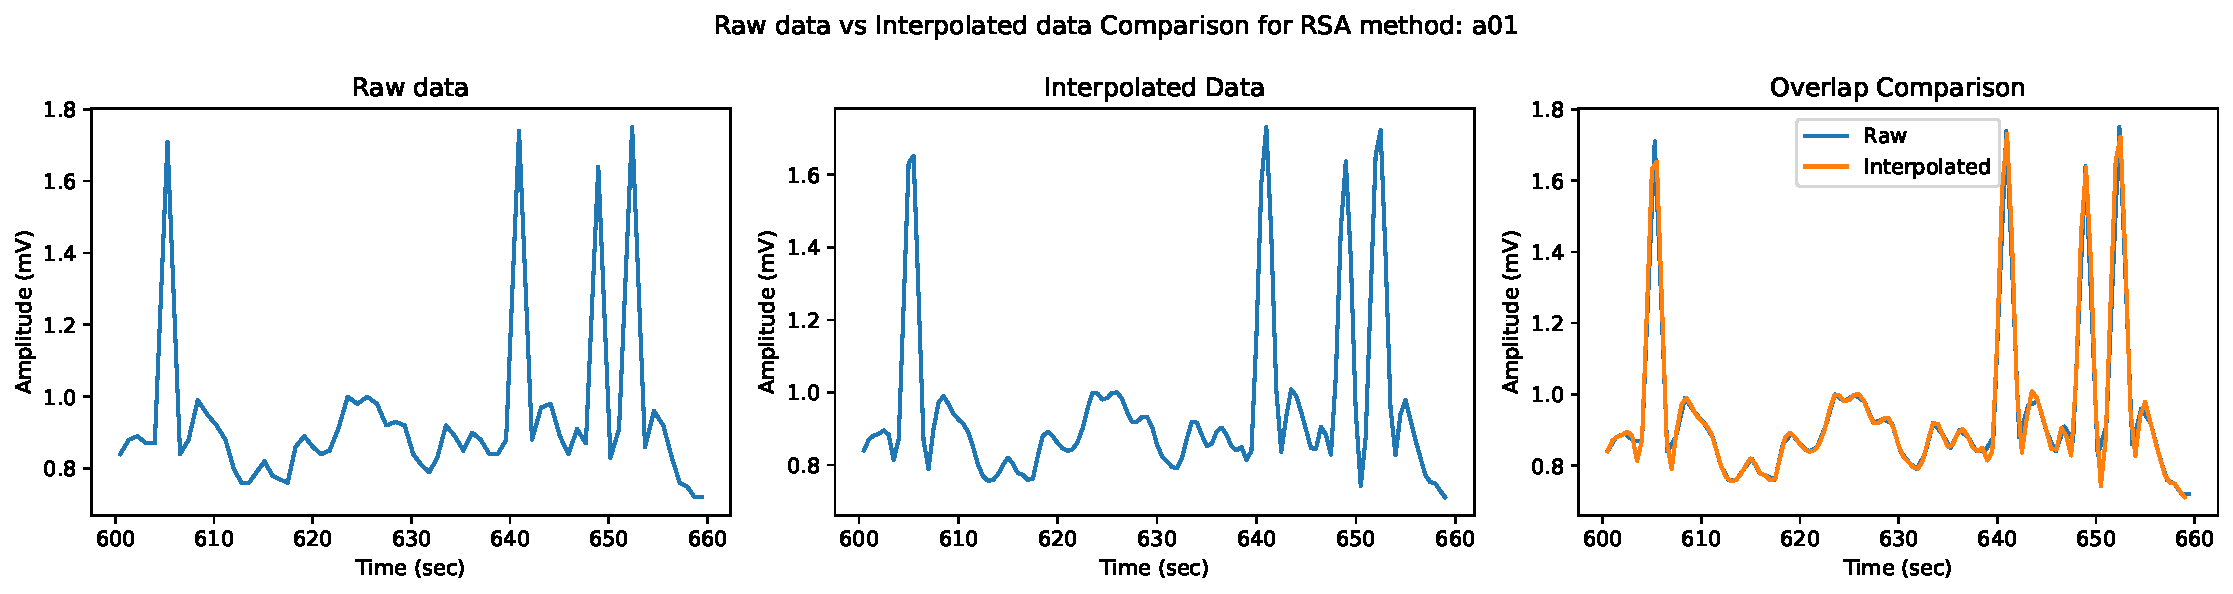
\includegraphics[width=\textwidth]{figures/RSA_method_interp.pdf}
    \caption{Raw data vs Interpolation comparison for RSA method}
    \label{fig:RSA_interp}
\end{figure}
\begin{figure}[H]
    \centering
    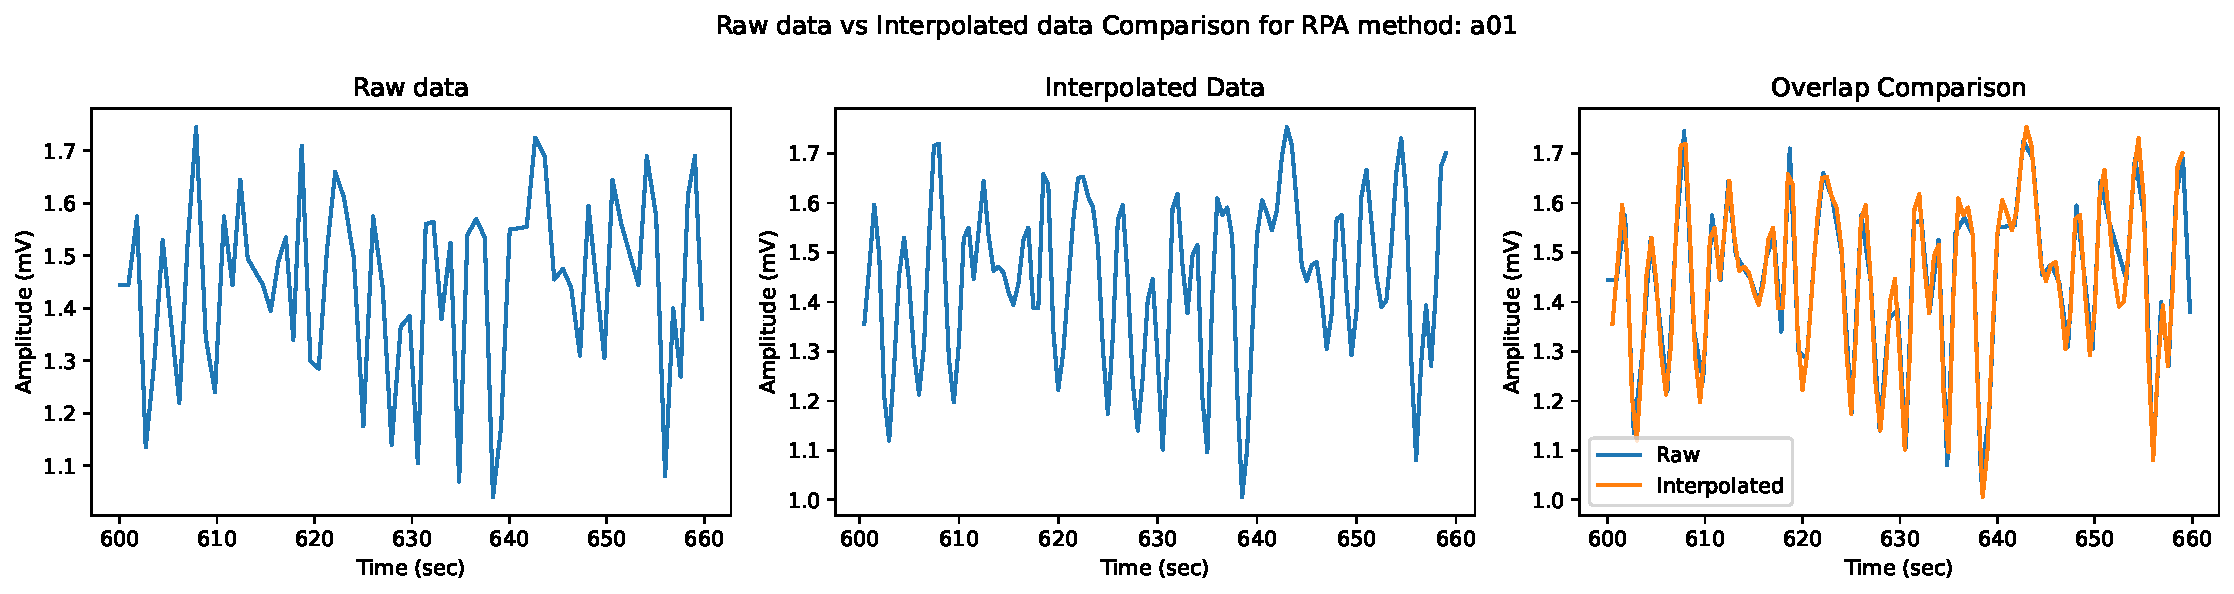
\includegraphics[width=\textwidth]{figures/RPA_method_interp.pdf}
    \caption{Raw data vs Interpolation comparison for RPA method}
    \label{fig:RPA_interp}
\end{figure}
The discrete Fourier Transform (FFT) is a method that decomposes a sequence of points into its frequency components. Per the Nquist 
Theorem, we consider frequencies that are multiples of 1/sample rate. For these frequencies, then when we consider 
a sample $(x_n), 1 \leq n \leq N$, where we have $N$ samples.The Discrete Fourier Transform for
frequency index $k$, is given by:
\[
X_k = \sum_{n=1}^N x_n \cdot e^{\frac{-2\pi ikn}{N}}. 
\]
Note that $X_k$ is often a complex number, where the magnitude corresponds to the amplitude, and the angle the phase. When plotting 
spectrums we are looking at the $|X_k|$ against its frequency $k$. When we refer to a Fast Fourier Transform this refers 
to an algorithm that computes the transform in the fastest known time complexity ($O(N\log N)$). 
\subsection{LombScargle Method}
The reference, \cite{VanderPlas2018}, provides a full description and discussion on the LombScargle Method, the method 
we implement is per SciPy, whose documentation is given by \cite{SciPyLombScargle}, the method SciPy implements is 
described by \cite{Zechmeister2009}. The basic idea is that the LombScargle 
Method is statistical, where each frequency $\theta$ is fitted to a function of the form,
\[
f_\theta(x) = a*\cos(\theta x) + b*\cos(\theta x) + c.
\]
The fitting is done via weighted least squares estimates. 
This method has no reliance on uniform time, and thus allows us to directly analyse the spectrum of non-uniform data without 
relying on first interpolating. Something worth considering when implementing this method is that as it is statistical thus there is a presence
of error in the estimation. 

\subsection{Method Comparison}
In Figures~\ref{fig:RSA},~\ref{fig:RPA} we can see a comparison 
of both spectrum analysis methods being applied to each of the RSA and RPA waveforms. The overlap plots show that clearly 
both analysis methods pick up on the same frequencies, however they do 
so with different amplitudes, in the RPA case the LomgScargle 
Method picks up on large frequencies, whilst in the RSA case LombScargle and 
FFT methods are similiar, with the FFT method amplitudes being slightly larger. 
These Figures indicate that both methods are viable, as they pick up similiar 
frequency peaks with similiar amplitude proportions (i.e amplitudes of frequency 
in relation to others within the same method). As a preliminary spectrum analysis
doesn't conclusively point towards one of the spectrum methods, we evaluate 
the Respiratory Rate Method employing both methods.

\begin{figure}[H]
    \centering
    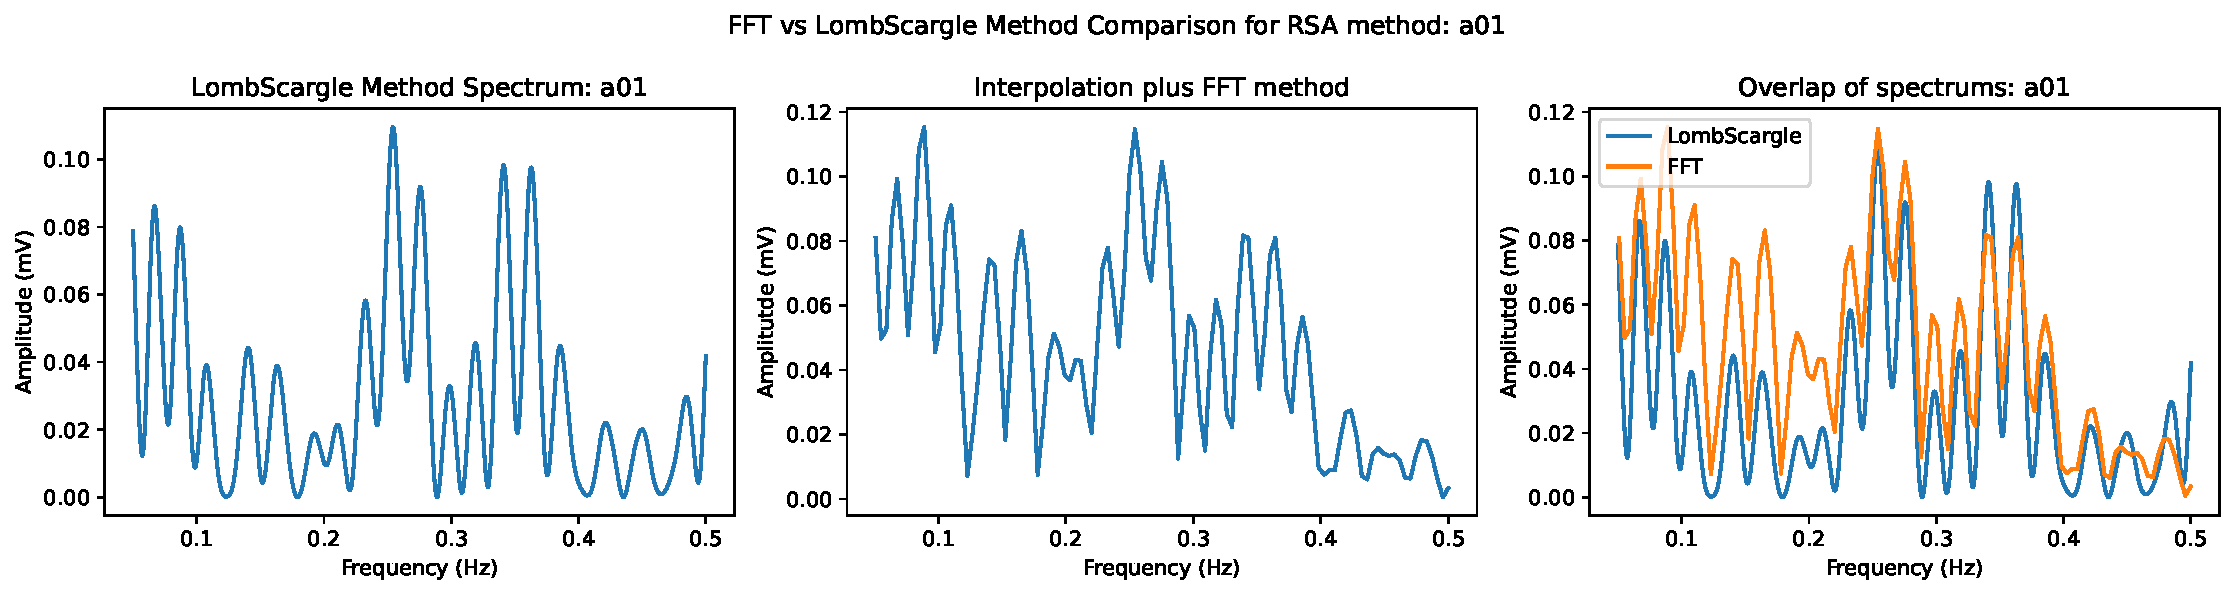
\includegraphics[width=\textwidth]{figures/RSA_method_spectrum.pdf}
    \caption{Spectrum comparison of LombScargle vs FFT based methods for RSA}
    \label{fig:RSA}
\end{figure}
\begin{figure}[H]
    \centering
    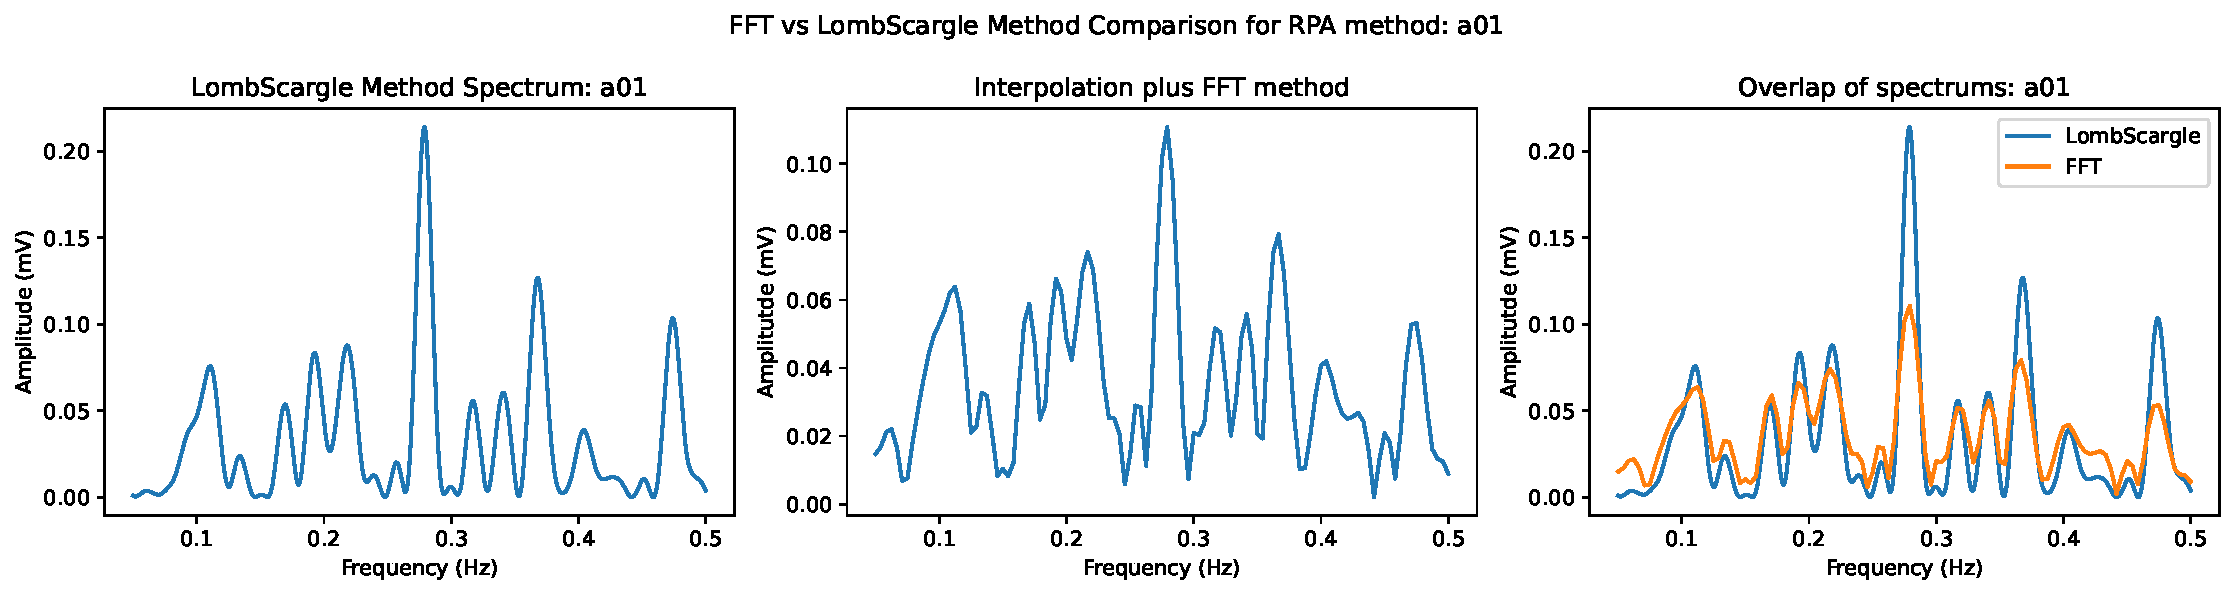
\includegraphics[width=\textwidth]{figures/RPA_method_spectrum.pdf}
    \caption{Spectrum comparison of LombScargle vs FFT based methods for RPA}
    \label{fig:RPA}
\end{figure}

In the following section we are going to produce Spectrograms, in producing these plots the time 
complexity of both methods becomes important, the Fast Fourier Implementation is $O(N\log N)$, whilst 
the LombScargle method is $O(NM)$, where $M$ is the number of frequencies, $N$ the number of data points. 
This difference becomes significant, and is why for compilation reasoning we focus largely on the FFT based method, 
which we shown to be valid. 


\section{RSA vs RPA Performance}
We begin evaluating RSA vs RPA methods by looking at spectrums, in Figure~\ref{fig:RPAvsRPA}, 
we can see in the overlap plots that both RSA and RPA methods, employing 
either the FFT or LombSCargle spectrum analysis pick up on similiar frequencies. 
However the a key thing to notice is in our 
expected Respiratory Rate interval (0.2 -0.33), RSA picks 
up on two frequency peaks whilst RPA only picks up on one, this is an
indication that the RPA method may be able to isolate a dominate frequency 
better. 

\begin{figure}[H]
    \centering
    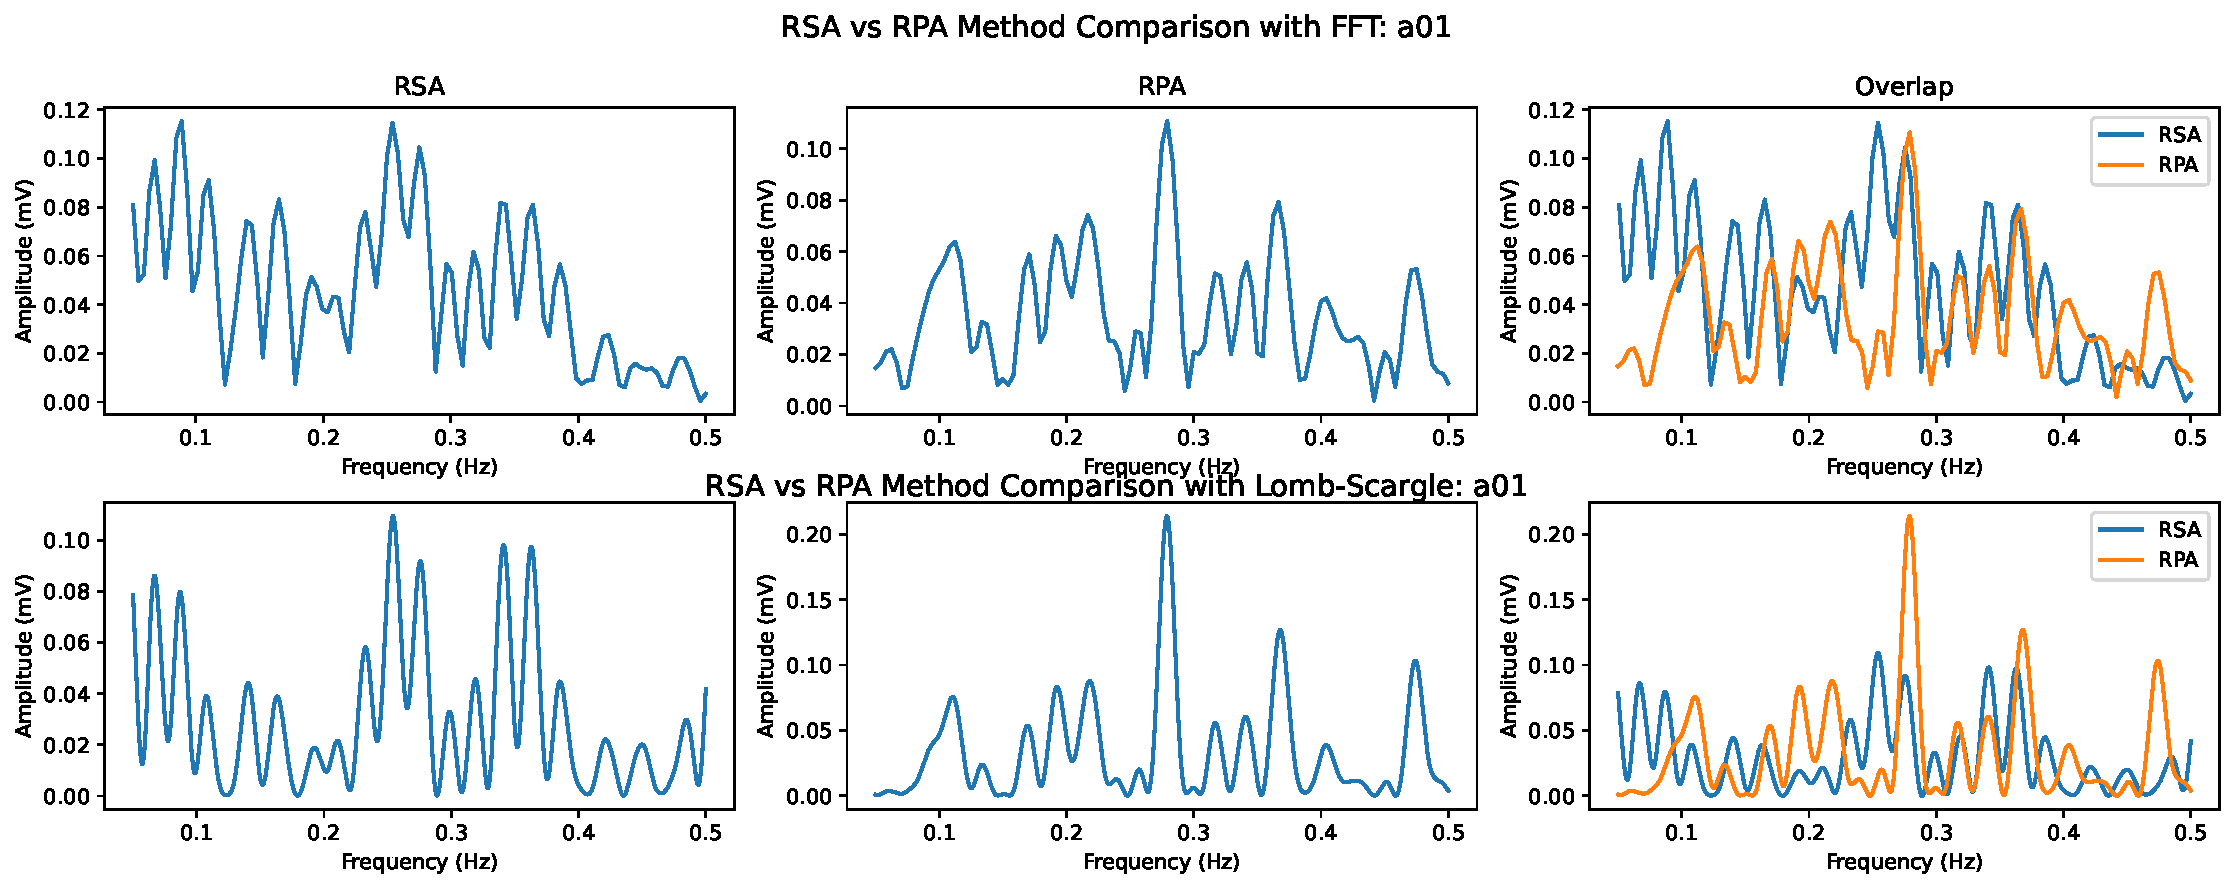
\includegraphics[width=\textwidth]{figures/RSA_vsRPA_spectrum.pdf}
    \caption{Spectrum comparison of RSA vs RPA method}
    \label{fig:RPAvsRPA}
\end{figure}

To better evaluate each methods we now focus on analysing Spectrograms, 
which tell us how the spectrum changes over time, as we expect Respiratory Rate to remain relatively 
stable \cite{braun1990respiratory}, we use spectograms to see if we can pick up on a consistent dominate frequency within the expected 
range. If we are able to, that would be a good indication of the methods ability to 
estimate the Respiratory Rate. In what follows the spectrograms work on a 60sec window, with 10 sec increments, i.e 
produces a spectrum every 10secs, based on a 60sec window of data (30 secs each side).  Figures~\ref{fig:RPAvsRPA_spec_FFT},~\ref{fig:RPAvsRPA_spec_lg} we can see
a Spectrogram over the first hour for each method, implemented with each analysis technique. 
Its clear in both figures that the RPA method picks up on a stronger dominate frequency sitting just below 
0.3HZ compared to the RSA method, which picks up a similiar frequency however with a weaker 
amplitude. 

\begin{figure}[H]
    \centering
    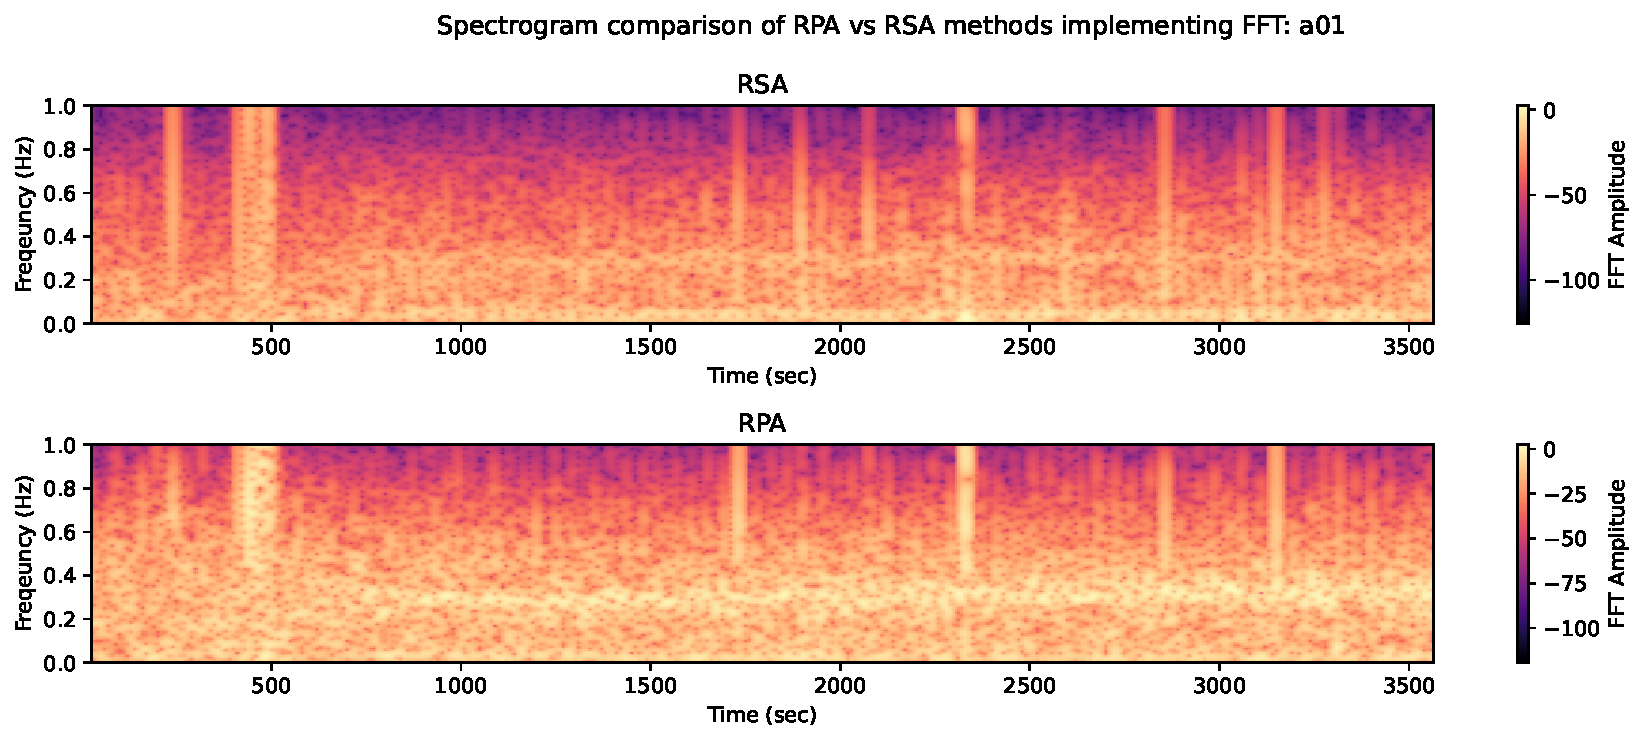
\includegraphics[width=\textwidth]{figures/RSA_vsRPA_spectrogram_FFT.pdf}
    \caption{Spectrogram comparison of RSA vs RPA method with FFT implementation}
    \label{fig:RPAvsRPA_spec_FFT}
\end{figure}


\begin{figure}[H]
    \centering
    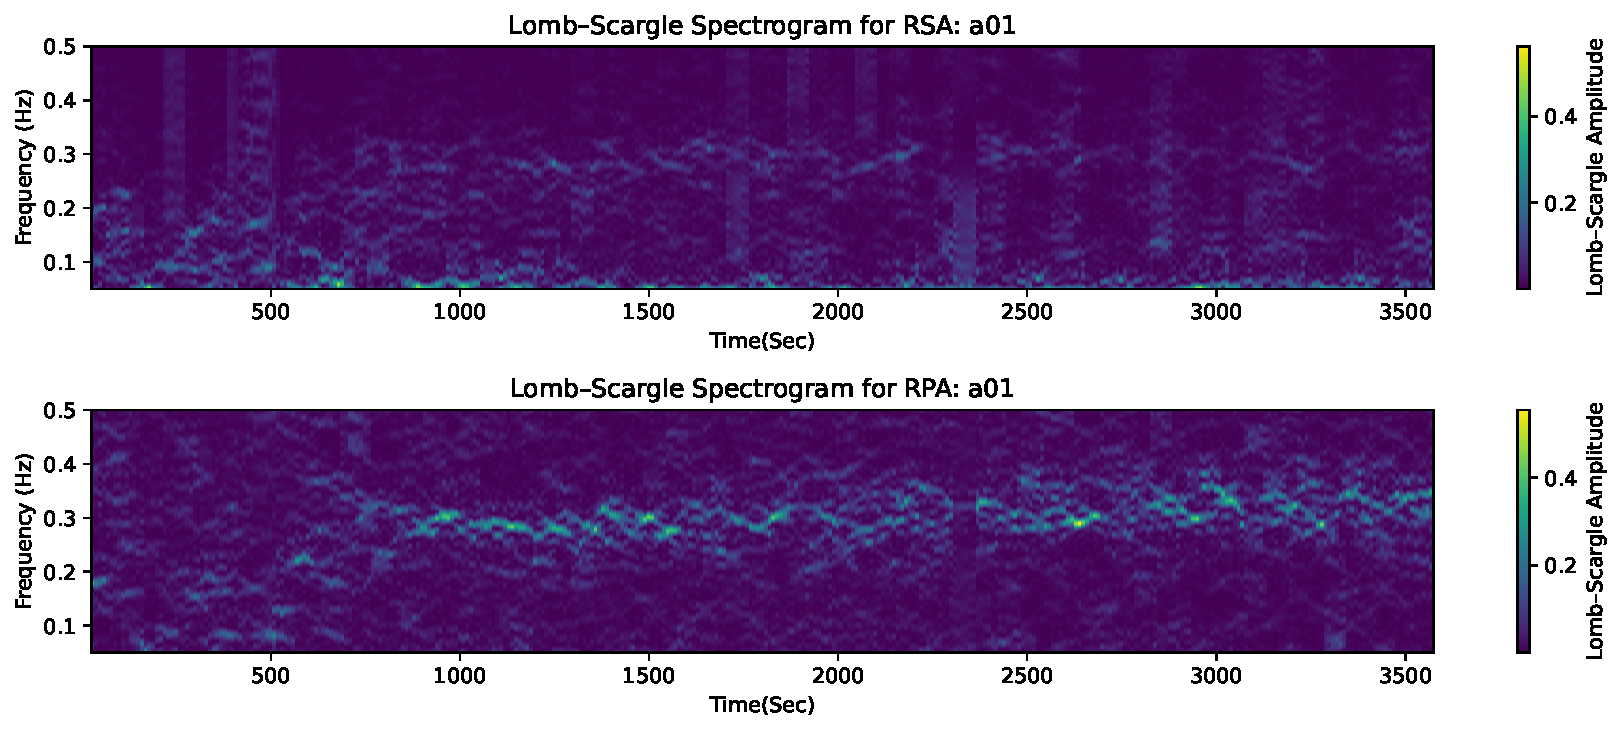
\includegraphics[width=\textwidth]{figures/RSA_vsRPA_spectrogram_lg.pdf}
    \caption{Spectrogram comparison of RSA vs RPA method with LombScargle implementation}
    \label{fig:RPAvsRPA_spec_lg}
\end{figure}

Thus far it appears that the RPA method seems to perform better than the RSA based method. 
We now explore the performance of the RPA method, with the FFT implementation as that had the 
clearest consistent dominate frequency in the Spectrograms above, whilst also being far less 
computationally expensive.  In Figure~\ref{fig:RPA_files_fft}
we can see the Spectrogram of the RPA method applied to our 8 test datasets. In the Figure 
its clear the method lacks robustness as it is only able to detect a dominate frequency 
pattern in the a01 data set, in the other 7 no clear pattern is visually distiniguishable.
This is indicative of the noise that is present, indicating that the RPA method 
needs to be made robust to noise, this makes sense as the method is based upon 
amplitudes, which would be highly sensitive to artifacts and noise affecting the ability 
of the method to pick up on the frequency associated with Respiratory Rate. 

\begin{figure}[H]
    \centering
    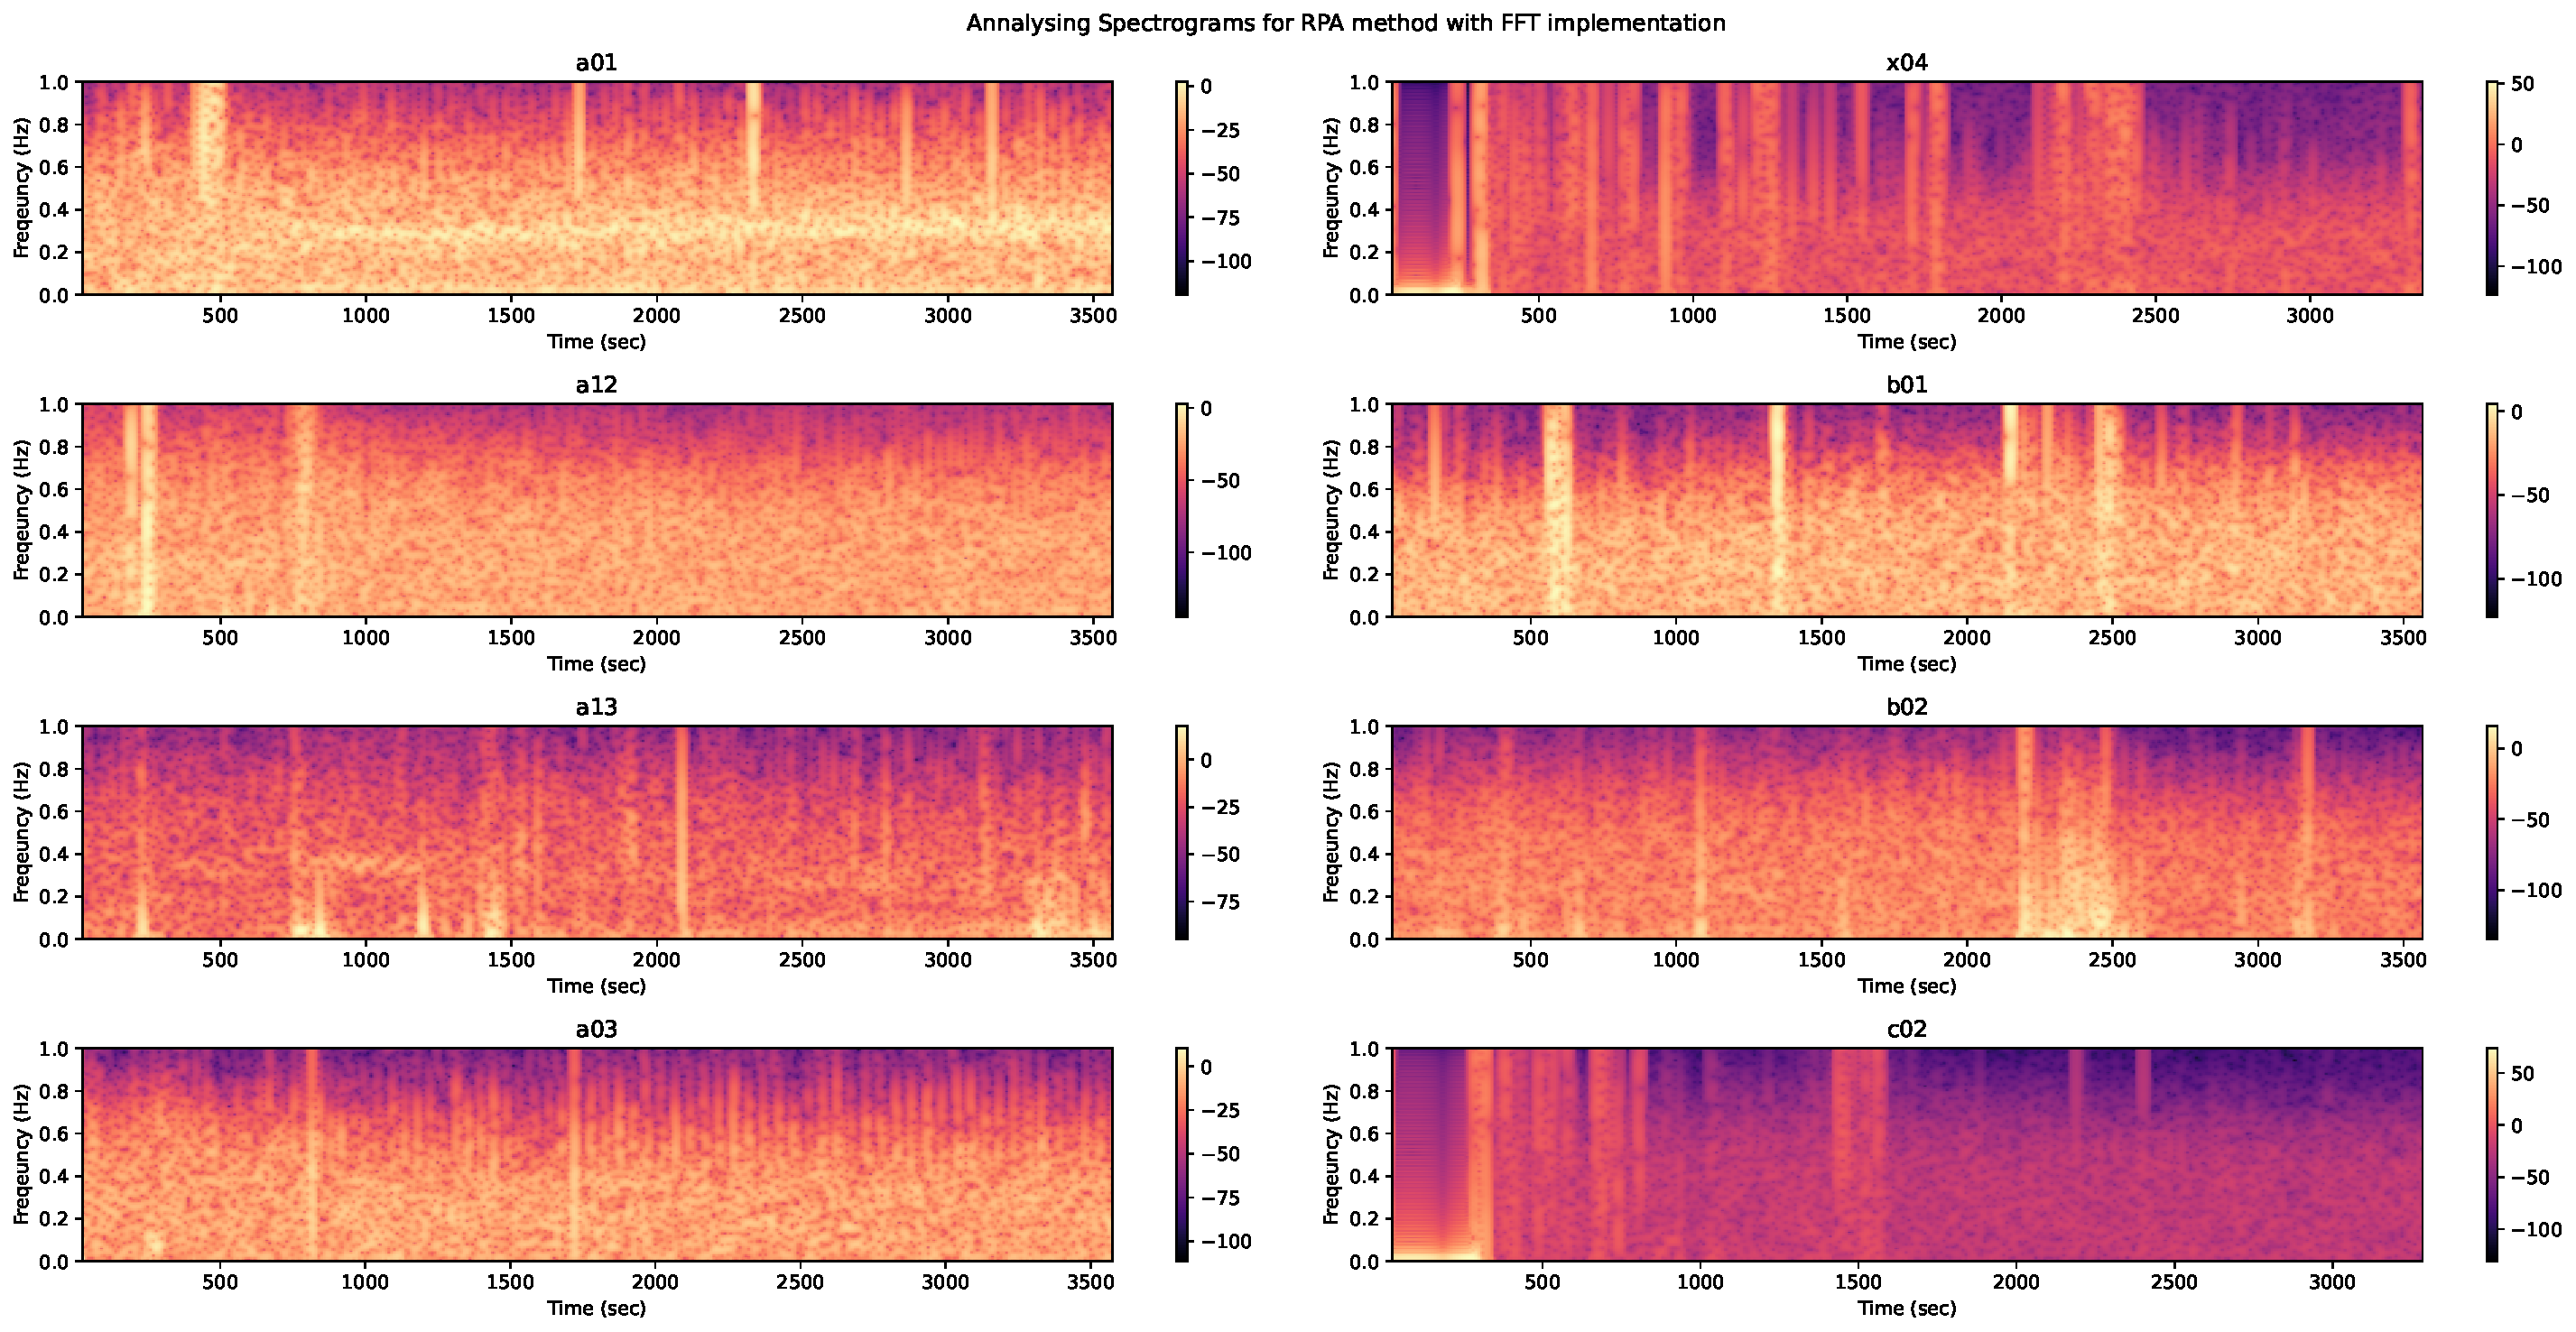
\includegraphics[width=\textwidth]{figures/RPA_spectrogram_files_FFT.pdf}
    \caption{Spectrogram comparison across datasets for RPA method with FFT implementation}
    \label{fig:RPA_files_fft}
\end{figure}

It is possible that the occurence of QRS complexes is less sensitive to noise,
so despite performing worse in the test case we now explore its performance, with FFT implementation, as shown 
in Figure~\ref{fig:RSA_files_fft}. 
\begin{figure}[H]
    \centering
    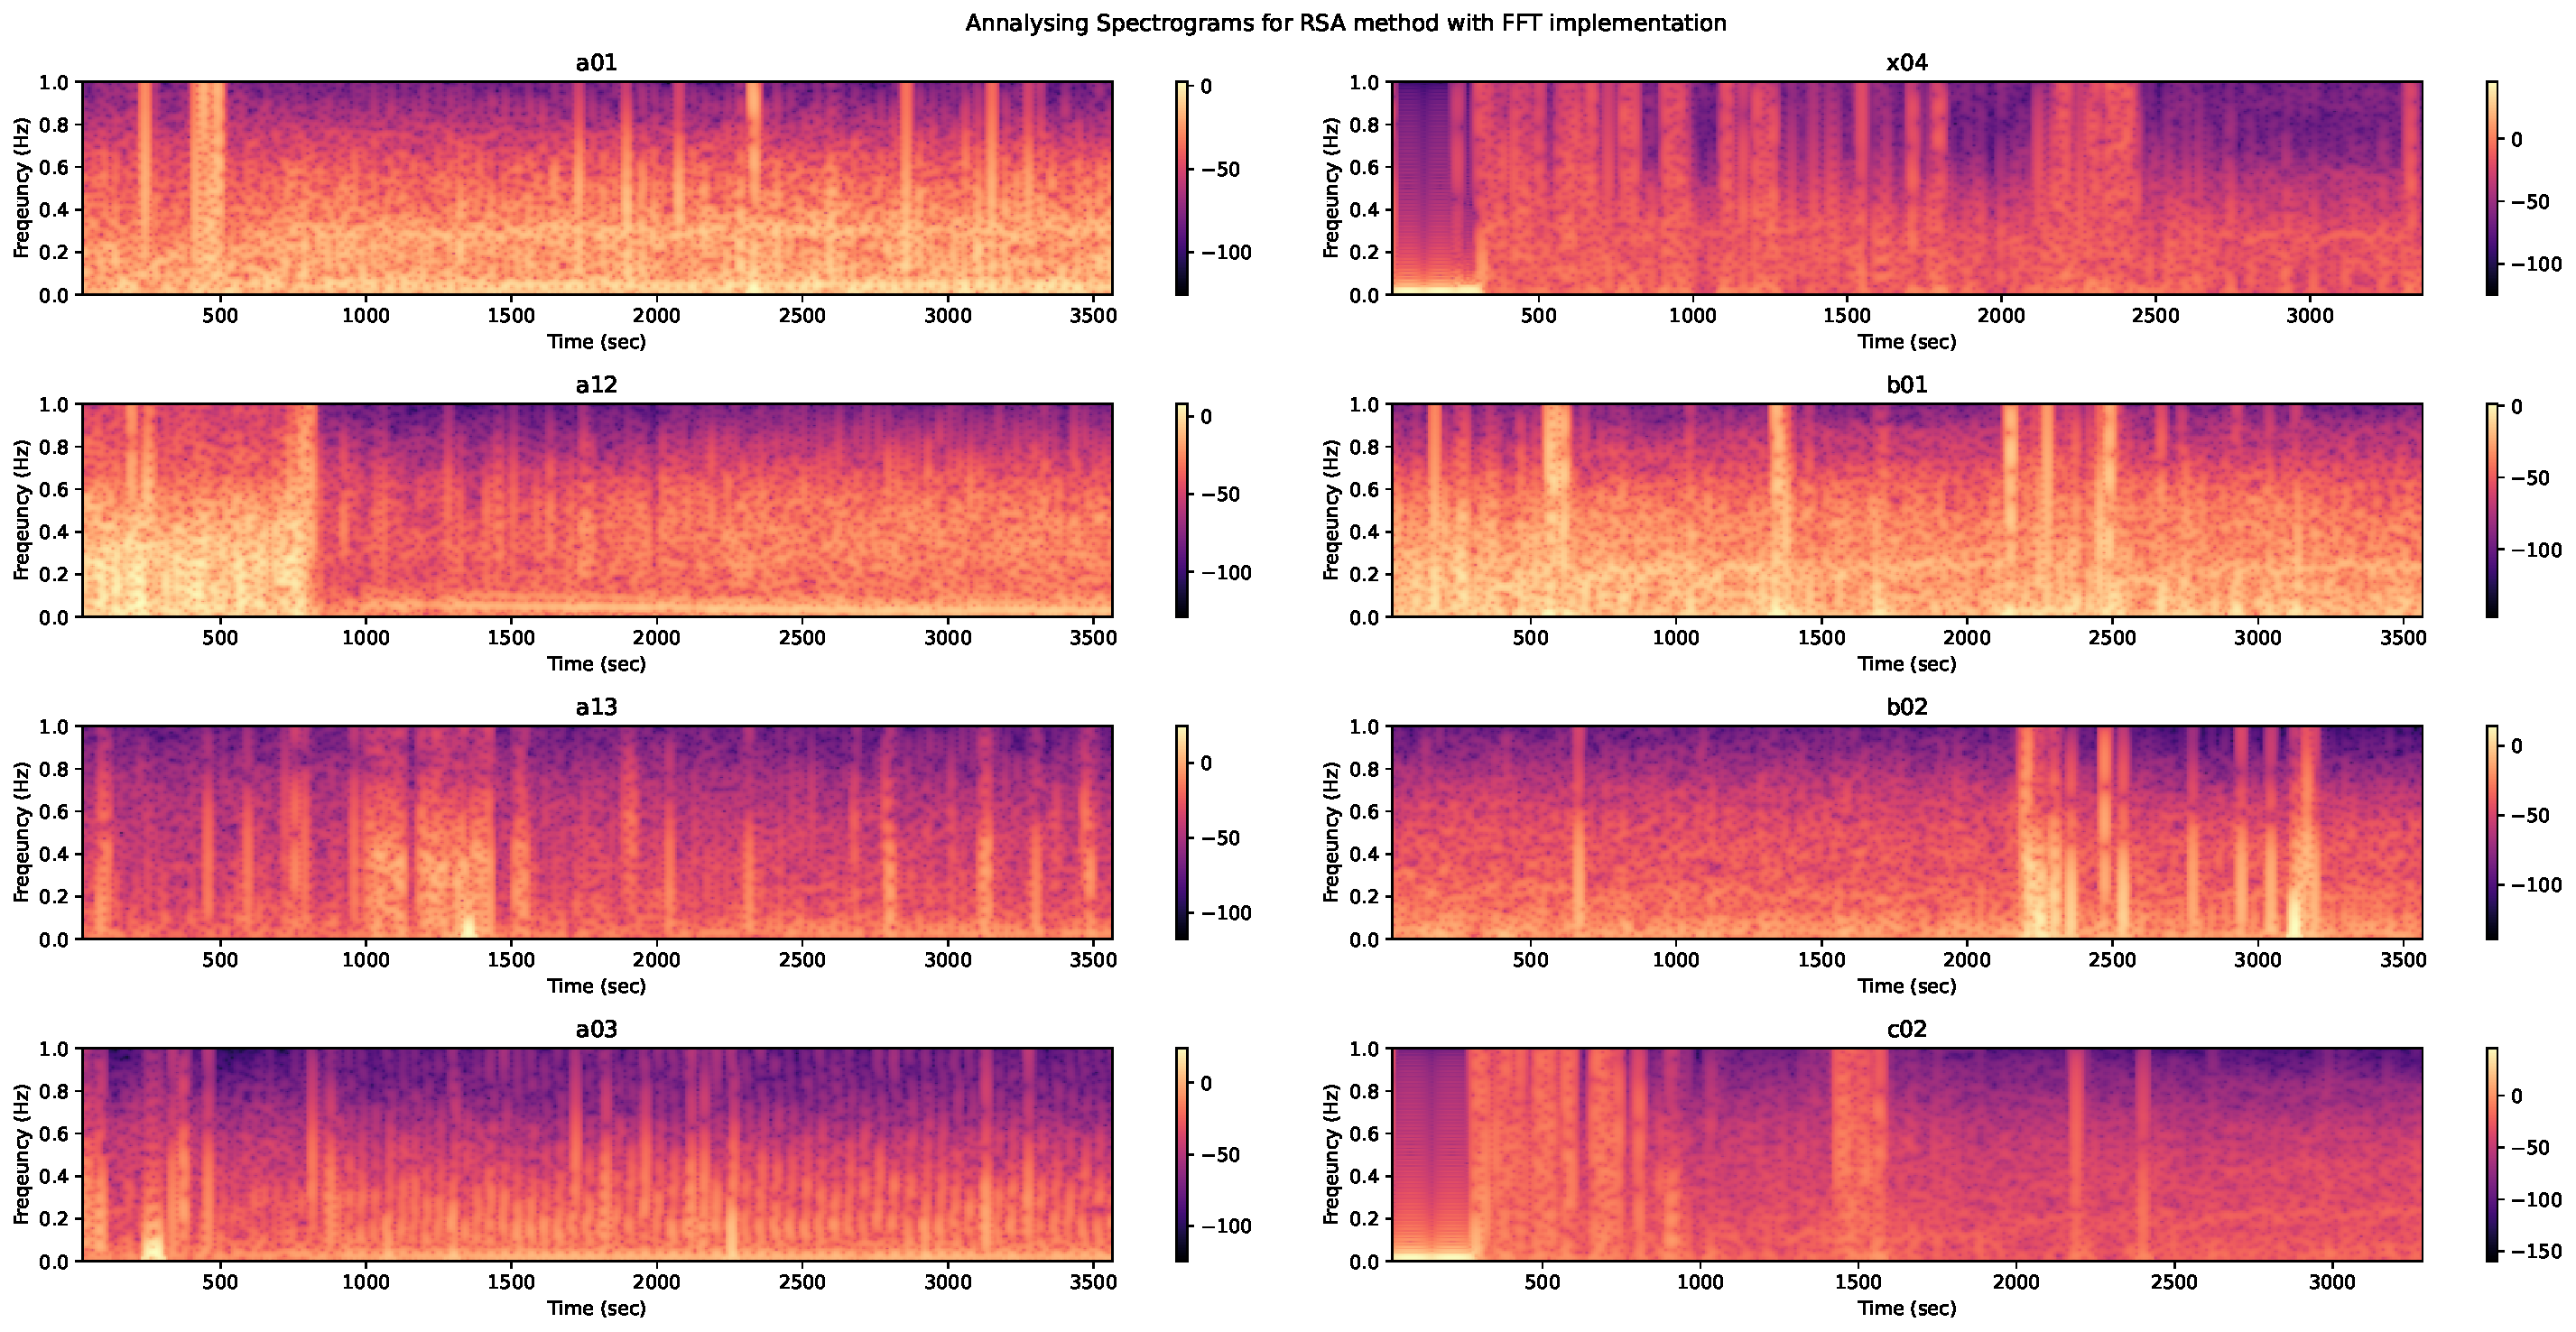
\includegraphics[width=\textwidth]{figures/RSA_spectrogram_files_FFT.pdf}
    \caption{Spectrogram comparison across datasets for RSA method with FFT implementation}
    \label{fig:RSA_files_fft}
\end{figure}
Looking at datasets b01, c02, b02 there are faint signs of a consistent 
frequency being picked up, most notably in dataset b01. This faint signal wasn't picked up 
by the RPA method, this indicates that whilst the RPA method may be better at picking up a stronger signal, 
it isn't as robust as the RSA method may be. \\
In the Figures above we have only compared the FFT based implementations, the reasoning is that as 
discussed the LombScargle method is more computationally expensive, as so producing and 
saving the Spectrograms is time and memory consuming, further the LombScargle method being 
statistical introduces error into the estimation. We saw that the interpolation 
method is very similiar in behaviour to the raw data providing validity for working with this method. 